\chapter{Background}
This chapter will introduce some necessary background knowledge on the target hardware platform, Java and the Java Virtual Machine, and JIT and AOT compilation.

\section{Wireless Sensor Networks and the Internet of Things}
Both Wireless Sensor Networks and Internet of Things are relatively new research areas. Both consider networks of connected devices that have to cooperate to achieve some goal. There is a large overlap between the two, but there are also key differences.

Wireless sensor networks is commonly understood to refer to networks of very resource-constrained devices. They are usually homogeneous, dedicated to a specific application, and in many cases battery powered. On the other hand, Internet of Things applications may contain the same class of resource-constrained devices but mix in more powerful ones as well. They may have a combination of battery- and mains powered devices. And the devices used may be a combination of devices dedicated to a particular task and smart devices that happen to be in the user's environment. One of the main challenges of IoT research is to develop ways to use the capabilities that are present in the smart devices around us to build new and useful applications.

It is this combination of heterogenous devices, and the need to reprogramme them to run new tasks that were not part of the original programming, that makes the platform independence and safe execution environment a VM may offer an attractive option.

While there is a wide range of IoT devices, they can be roughly divided in two categories. We will describe the capabilities and limitations of each of them below. 


\subsection{High-end IoT devices}
Another decade of miniaturisation since the start of WSN research has allowed us to scale down devices capable of running a normal OS stack, to the size of a few centimetres. Some of the most popular examples include the Raspberry Pi, with the Raspberry Pi Zero being only 65x30mm, and the Intel Edison at 35.5x25mm.

These devices have capabilities similar to that of desktop PCs only a few generations ago. They can run a normal operating system like Linux and all the standard protocols and tools that come with it. Compared to the traditional resource-constrained sensor nodes, the can perform much more complex tasks, but the smallest devices in this class are still significantly larger than the smallest sensor nodes, more expensive, and most importantly, consume significantly more power.
%TODO add this reference http://ieeexplore.ieee.org/document/7969879/

Since devices in this class are capable of running normal, well established VMs, we do not consider them in this dissertation, but instead focus on the second class of devices: sensor nodes.

\subsection{Resource-constrained sensor nodes}
The second class of devices, wireless sensor nodes, are distinctly less powerful. They are designed to be deployed at low cost and potentially in large numbers, and are capable of running for weeks or months on a single battery charge. As a typical example, the MICAz node \cite{CrossbowTechnology} uses only 30mA when active and 16uA in sleep mode. More recently, the Arduino family of devices, based on similar hardware, has led to a very active community of both research and hobby projects.

While an enormous number of different hardware platforms have been developed, the components they use come from a limited set. Two of the most popular families of CPUs used in these platforms are the Atmel AVR and Texas Instruments MSP430. Both families of CPUs come in a large number of variations with different amounts of memory, IO ports, and physical packages, but the underlying architecture is similar for all. Table \ref{tbl-ATmega128-msp430f1611} lists the main characteristics for two popular member for both families, the ATmega128 and the MSP430F1611. Below we will describe the most important properties for this class of devices that are relevant to the work in this dissertation.

\begin{table}
\caption{Main characteristics of the ATmega128 and MSP430F1611 CPUs}
\label{tbl-ATmega128-msp430f1611}
    \begin{threeparttable}
    \begin{tabular}{lrr}
    \toprule
                                           & ATmega128 \cite{Atmel:ATmega128Datasheet, Atmel:AVRInstructionSetManual}   & MSP430F1611 \cite{TexasInstrumentsIncorporated:MSP430F1611Datasheet, TexasInstrumentsIncorporated:MSP430x1xxUsersGuide} \\
    \midrule
    \midrule
    Number of registers                    & 32           & 12            \\
    Register size                          & 8-bit        & 16-bit        \\
    RAM                                    & 4KB          & 10KB          \\
    Flash                                  & 128KB        & 48KB          \\
    Frequency                              & up to 16MHz  & up to 8MHz    \\
    Simple instruction cost                & 1 cycle      & 1 cycle       \\
    Memory access cost                     & 2 cycles     & 2 to 6 cycles \\
    Branch cost (taken/non-taken)          & 2 / 1 cycles & 2 cycles      \\
    Active power consumption\tnote{a}      & 7.5mA        & 4.3mA         \\ % MSP430 current calculation: 8*(600+(210*(2.7-3)))=4296 uA
    Deep sleep power consumption           & 0.3uA        & 0.2uA         \\
    Can execute code from                  & Flash        & Flash and RAM \\
    \bottomrule
    \end{tabular}
    \begin{tablenotes}
        \item[a] at 8MHz and 2.7V
    \end{tablenotes}
    \end{threeparttable}
\end{table}

\paragraph{Memory}
Memory is split into persistent flash memory for code, and volatile RAM for data. The MSP430 CPUs have a von Neumann architecture and can execute code from both, while the AVR's Harvard architecture can only execute code from flash memory. Flash memory is typically in the range of 16KB to 256KB, while RAM, which consumes energy even in sleep mode, is restricted to up to 10KB. There are no caches, and since both memories are on chip, access times are constant and take only a few cycles.

\paragraph{Simple architecture}
These CPUs achieve their extremely low cost and power consumption by restricting themselves to very simple design. Each instruction costs a fixed number of cycles, varying only for taken or non-taken branches. Since most instructions only take one or two cycles, there is no pipelining or need for branch prediction. There is also no memory management unit or protection rings, and no floating point support.

\paragraph{Operating system}
The severe resource restrictions on these devices mean that a normal layered architecture with an OS, networking stack, and applications running on top of that is not possible. The closest thing to a widely accepted OS for sensor nodes is TinyOS \cite{Levis:2004ws} which provides several basic services for IO, communication and task management. Contrary to a normal OS, TinyOS doesn't 'load' an application, but is in fact more like a library that is statically linked with the application's code to form a single binary which is then programmed into the node's flash memory. Thus, sensor node applications are often a single binary, running directly on the CPU.

Several systems exist that allow over the air reprogramming of applications \cite{Quadri:2014wr}. In some cases these allow the entire application code to be replaced, including the reprogramming protocol itself \cite{Reijers:2003ww}. In other cases the reprogramming system may be permanent and include other basic services, which is more close to an operating system. Even in these cases the restricted amount of flash memory means that such a system cannot afford to waste large amounts of memory on library functions that may never be used by the application, so the services provided by such an 'operating system' are quite restricted, leaving much of the low level work to the application.

A number of sensor node virtual machines have also been developed that allow the application to be updated remotely. These obviously provide a higher level of abstraction from the underlying hardware. However it is important to note here that these virtual machines are not an extra layer, between a lightweight OS and the application, but usually \emph{replace} the OS entirely, so the VM runs directly on the CPU. This kind of cross layer optimisation, or complete merging of layers is typical of many sensor networks.

\section{The Java virtual machine}
Next, we will briefly introduce the Java virtual machine, and describe some of the details relevant to this work.

The first public release of Java was in 1995. It consists of two separate but related parts: the Java programming language, and the Java virtual machine (JVM): an abstract machine specification, running programmes written in JVM bytecode. Since the release of Java, several other languages have been developed that compile to JVM bytecode and can run on the same virtual machine.

It was quickly adopted by web browsers to run interactive \emph{applets}. Two key properties of Java contributed to this success:
\begin{itemize}
    \item Implementations of the JVM could be built for any hardware platform, so the same applet could be run in any browser, regardless of the hardware it was running on.
    \item It allowed users to safely run applets from untrusted sources since the virtual machine ran applets in a 'sandboxed' environment with access to only those system resources explicitly allowed by the user.
\end{itemize}

For stand alone desktop applications Java also became popular because was an easy to learn, object oriented, garbage-collected language that allowed for a higher level of programming than C or C++, all of which boosted developer productivity.

\subsection{JVM bytecode}
Compared to other widespread desktop VMs such as Lua, Python and .Net, Java's bytecode is very simple. Java is a \emph{stack-based} virtual machine, as opposed to a \emph{register-based} virtual machine: almost all operations take their operands from an operand stack, and push their results back onto it. For example, Listing \ref{lst-basic-jvm-bytecode-example} shows how the statement \mycode{a=b+c;} may be translated into JVM bytecode. First, \mycode{a} and \mycode{b} are loaded onto the stack, the \mycode{IADD} instruction then pops these operands from the operand stack and pushes the sum back onto it, and finally \mycode{ISTORE} stores the result back into a local variable.

\begin{listing}
    \centering
    \begin{minted}{java}
    //JVM instruction     // JVM stack

    ILOAD_1               a
    ILOAD_2               a   ,   b
    IADD                  a+b
    ISTORE_0
    \end{minted}
\caption{JVM bytecode for \mycode{a=b+c;}}
\label{lst-basic-jvm-bytecode-example}
\end{listing}

By far the largest number of instructions, 99 out of 206, are for loading or storing data to and from the operand stack. These come in different flavours for different datatypes: \mycode{ILOAD} loads an int, while \mycode{BLOAD} loads a byte onto the stack. There 53 are simple arithmetic or bitwise operations, such as \mycode{IADD} in the example, also in different variations for different datatypes. There 39 for branches and method invocations, and 15 for various other tasks such as creating new objects and throwing exceptions.

Each JVM bytecode is encoded as a single byte. Some are followed by some operands, for example the method to call, or the type of object to create, but most are not. This very simple instruction set makes it a suitable basis for a sensor node VM, where we don't have the resources to process anything much more complicated.

\subsection{Memory}
\label{sec-background-jvm-memory}
The JVM stores information in three different places:
\begin{itemize}
    \item The heap: objects and arrays are stored here, and automatically garbage-collected when no longer used.
    \item The stack frame: each method's stack frame contains a section for that method's operand stack, and for its local variables.
    \item Global variables: static variables that are allocated globally when a class is loaded (we ignore \mycode{ThreadLocal} variables since they are not supported in our VM).
\end{itemize}

\begin{figure}
\centering
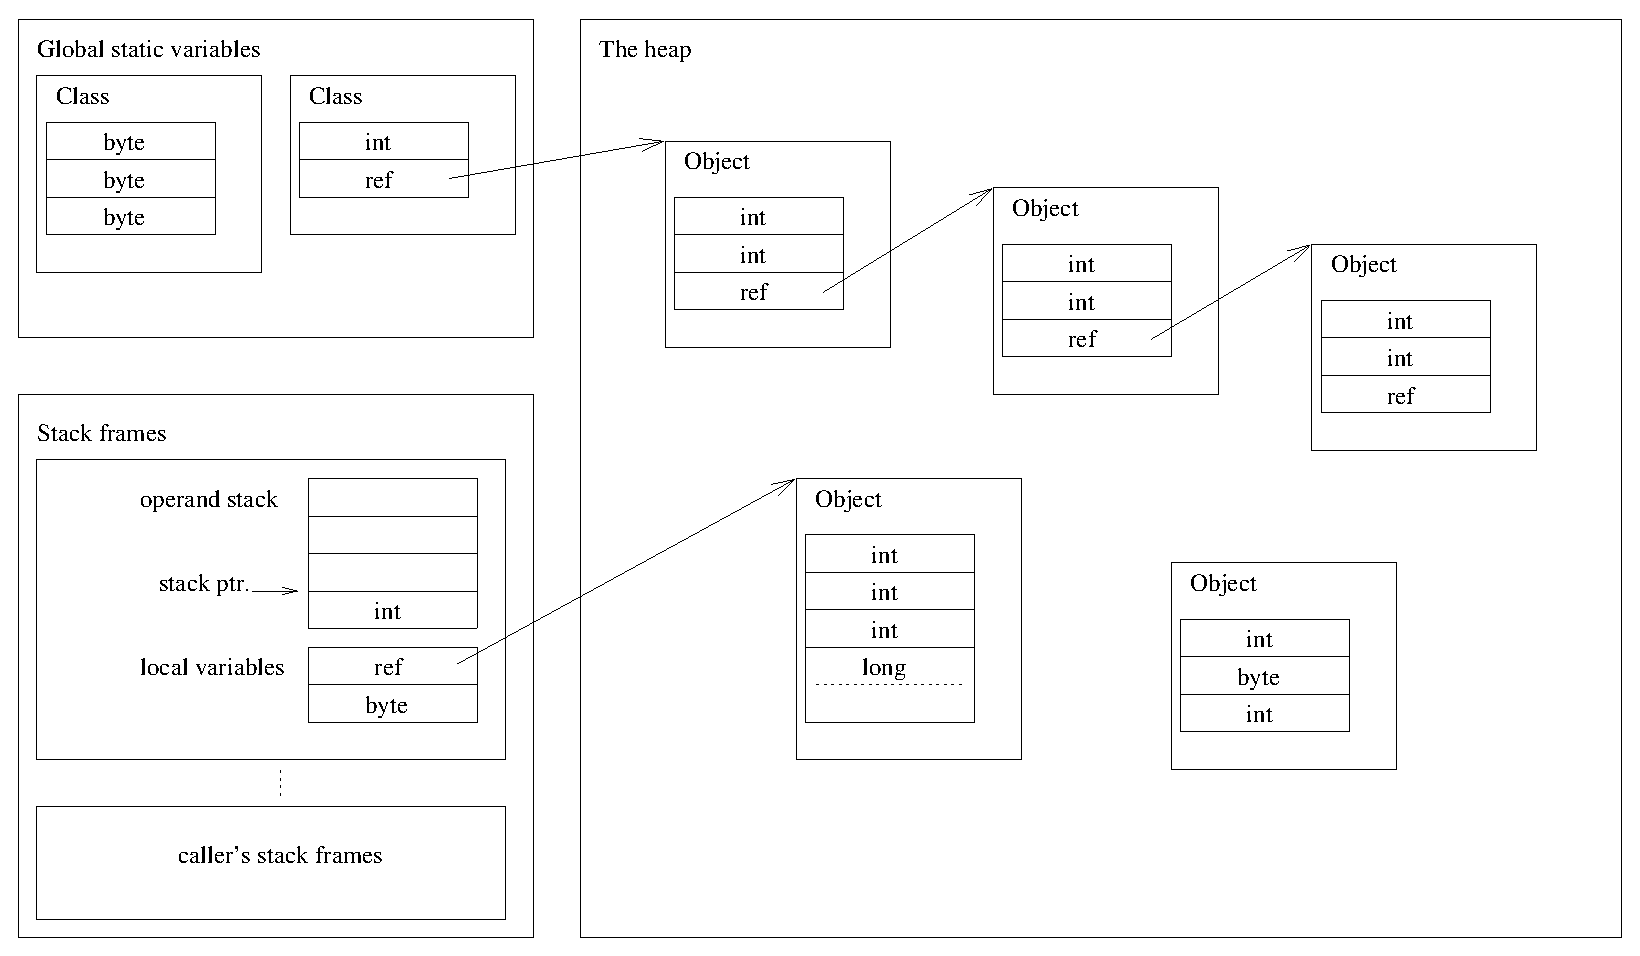
\includegraphics[width=\linewidth]{jvmmemory.eps}
\caption{Highlevel overview of JVM memory design}
\label{fig-jvm-memory}
\end{figure}

The JVM is a 32-bit machine. All the places where data may be stored, objects on the heap, operand stacks and local variable slots, and a class' static variables, are essentially a block of 32-bit wide slots. 64-bit \mycode{long} and \mycode{double} types occupy two slots on the operand stack of local variable space, while the shorter \mycode{byte}, and \mycode{short} types are sign-extended and stored as a 32-bit value.
  
Figure \ref{fig-jvm-memory} shows a graphical representation of this. An important difference with languages such as C, Pascal or C\# is that in JVM the only value types are the various integer types, and \emph{reference}. There are no compound types like a C \mycode{struct} or Pascal \mycode{record}. Object live in heap, and only there, and the operand stack, and local, static or instance variables only contain references to objects.

\subsection{Sandbox}
A sandbox is a security mechanism for isolating a process from the environment in which it runs. They can be used to run code from untrusted sources, without risk of harm to the host machine or other applications running on it.

In the JVM's case, programmes are written to run on the abstract JVM machine model. Besides providing platform independence, this also means JVM programmes have no knowledge of the hardware platform they will be running on. All communication with the outside world happens through the Java standard library classes implemented by the JVM in native code, which gives the virtual machine firm control over the resources an application may access.

In addition, the JVM will verify the bytecode at load time to make sure it is well formed and adheres to the JVM standard \cite{Lindholm:2017vu}. It performs many checks, for example that branches are within the bounds of the code array for the method, and branch to the beginning of an instruction, that execution cannot fall off the end of the code, that no instruction can access or modify a local variable at an index greater than or equal to the number of local variables that its method indicates it allocates, that, the exact stack depth and type of values on a method's operand stack is known at any point and doesn't over- or underflow, etc.

\subsection{WAT, AOT, and JIT compilation}
While the popularity of Java rose quickly after its introduction, it also very quickly got a reputation to be slow. As Tyma put it in 1998 "The plain truth is: Java is slow. Java isn't just slow, it's \emph{really} slow, \emph{surprisingly} slow. It is 'you get to watch the buttons being drawn on your toolbar' slow." \cite{Tyma:1998vj}.

The main reason is all early implementations of the JVM were interpreters. An interpreter executes a program by retrieving instructions from memory one at a time, and then executing them. An outline of what a typical interpreter's main loop looks like is shown in Listing \ref{lst-interpreter-loop-outline}. For each instruction, the VM needs to (i) retrieve the bytecode at the current programme counter, (ii) increment the programme counter, (iii) jump to the correct case label, (iv) execute the instruction, and (v) loop for the next iteration.

\begin{listing}
    \centering
    \begin{minted}{C}
    while (true) {
        opcode = bytecode[pc];
        pc++;
        switch (opcode) {
            case ILOAD_0: ...
            case ILOAD_1: ...
            ...
    }
    \end{minted}
\caption{Outline of a typical interpreter loop}
\label{lst-interpreter-loop-outline}
\end{listing}

Since most instructions are very simple, for example simply adding two operands, the relative overhead from these steps is very high. Interpreters spend most of their time on the interpreter loop, and only a fraction of the time on actually executing the JVM instructions.

Thus, a common approach to improve JVM performance is to translate the bytecode to the native machine code of the target platform before executing it. Three main approaches exists, which differ in at what point the bytecode is translated to native code.

\paragraph{Compile time}
Borrowing the term from Proebsting et al., Way-Ahead-of-Time (WAT) compilers translate to native code during or directly after compiling the Java sources \cite{Proebsting:1997wg}. Some systems first translate to C \cite{Dean:1996wb}, which is then compiled using normal optimising C compilers. 

Regardless of which approach is chosen, the result is a native binary for the target platform, rather than JVM bytecode. The advantage of this approach is that ample time and resources are available during at compilation time so highly optimised code can be produced. However, the downside is that the resulting code is no longer platform independent or guaranteed to be properly sandboxed.

\paragraph{Load time}
A second group of compilers translate bytecode to native code at load time. In these cases the entire application is translated to native code, before it is run. Therefore, they are usually called Ahead-of-Time (AOT) compilers. An example of this approach is early versions of Android's ART runtime, which translates an app the moment it is downloaded onto a device (although it since has mixed in JIT techniques as well, discussed below).

The advantage is that it combines the advantage of WAT, being able to spend considerable resources on optimisation, with platform independence and a guaranteed sandbox, since the translation is now fully under control of the device running the application, rather than the device compiling it. A downside is that the initial translation adds to the time it takes to load or install an application.

\paragraph{Run time}
Finally, the last group of compilers, called Just-In-Time (JIT) compilers, incrementally translate the bytecode to native code while the application is running. While an obvious downside is that this may initially slow down the application while it is translating bytecode at run time, a JIT compiler can take advantage of the observed run-time characteristics to make better optimisation decisions or do more aggressive optimisations that may have to be rolled back if some preconditions no longer hold. For example inlining a virtual method as long as only a single implementation is loaded \cite{Ishizaki:2000vv}.







